\section{Makefile}

In eine Makefile können Abhängingkeiten definiert werden\\
Wenn eine Datei geändert wurde, dann werden alle Operationen ausgeführt mit den Dateien, welche von
dieser geänderten Datei abhängen

\textbf{Il makefile viene eseguito dal basso verso l'alto!}

\subsection{Variabili}
Le variabili vengono definite come \texttt{NAME = valore} e richiamate con \texttt{\$(NAME)}. 
Esempio:
\begin{lstlisting}[language=make]
CC = clang
CFLAGS = -c -Wall
\end{lstlisting}

\subsection{Regole e Dipendenze}
La sintassi fondamentale è:
\begin{center}
\texttt{Target: Dipendenze} \\
\texttt{\quad [TAB] Comando Shell}
\end{center}

\begin{itemize}
    \item Il comando viene eseguito solo se una dipendenza è più recente del target.
    \item Il simbolo '\texttt{\$@}' rappresenta il nome del target corrente.
    \item È obbligatorio l'uso del tasto TAB per i comandi.
\end{itemize}

\subsection{Esempio Pratico}
\begin{center}
    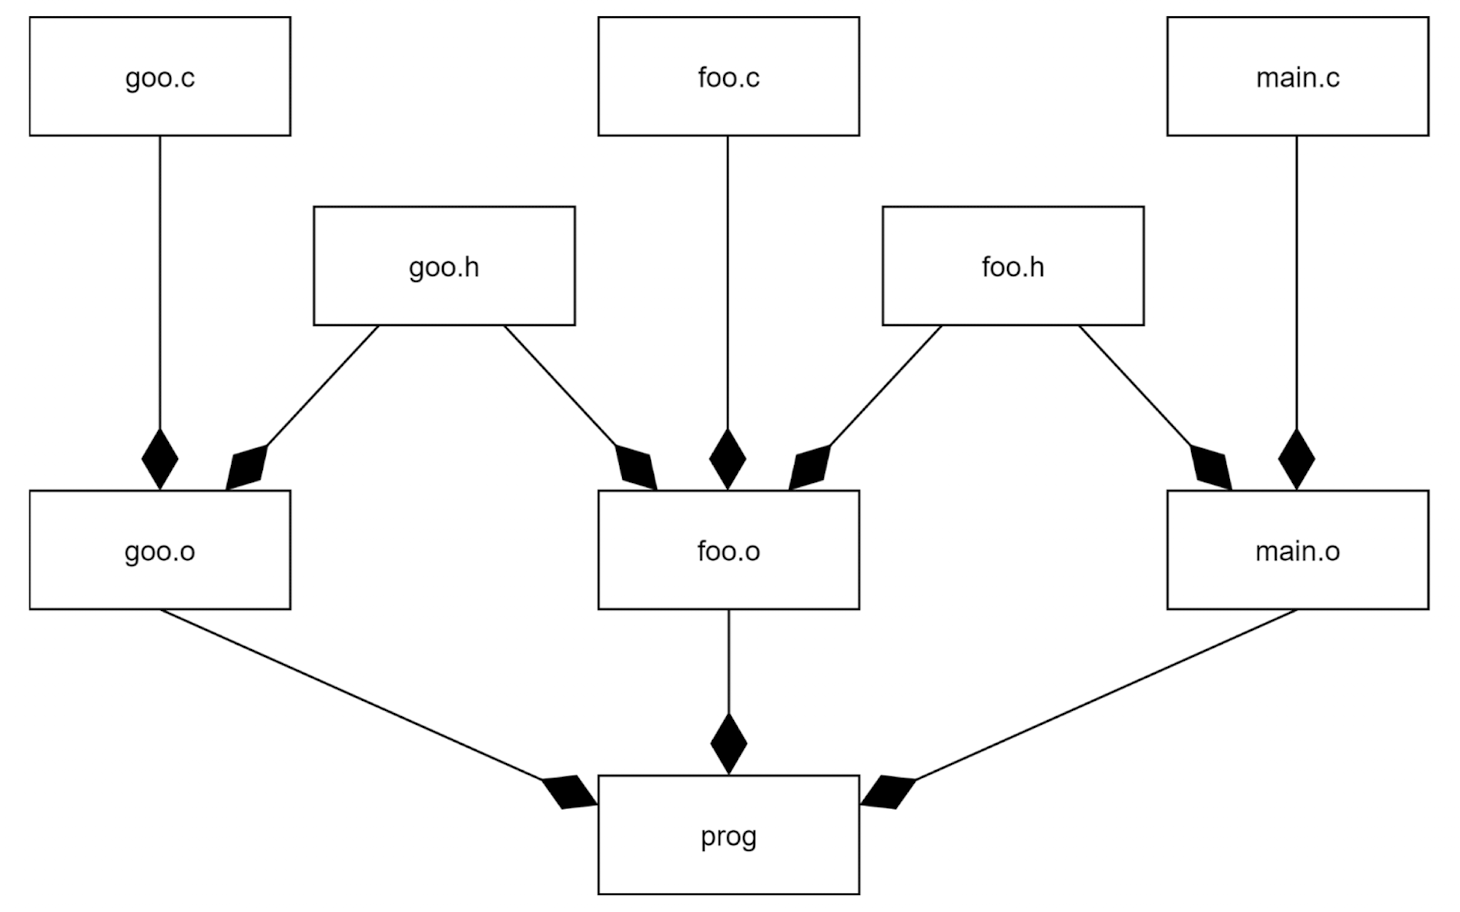
\includegraphics[width=0.78\columnwidth]{images/dateien_abhaengigkeiten.png}
\end{center}\vspace{-1.5em}

\lstinputlisting[language=makefile]{code/05_makefiles/makefile}